\documentclass{article}
\usepackage{enumitem}
\usepackage{graphicx}
\usepackage[utf8]{inputenc}
\usepackage{listings, xcolor}
\usepackage{url}
\usepackage{todonotes}

\lstset{
tabsize = 4, 
showstringspaces = false,
numbers = left, 
commentstyle = \color{green}, 
keywordstyle = \color{blue}, 
stringstyle = \color{red}, 
rulecolor = \color{black},
basicstyle = \small \ttfamily , 
breaklines = true,
numberstyle = \tiny
}

\graphicspath{ {./images/} }
\author{Kenneth Hansen}
\title{Latex assignment - Part Two}

\begin{document}
\maketitle
\thispagestyle{empty}
\tableofcontents

\clearpage 
\section{Introduction \LaTeX}
\inputencoding{utf8}
These are dannish characters øæå

\subsection{Graphics - subsection}

\begin{figure}[!h]
  \centering
  \begin{minipage}[b]{0.4\textwidth}
    \caption{This is a monkey}
    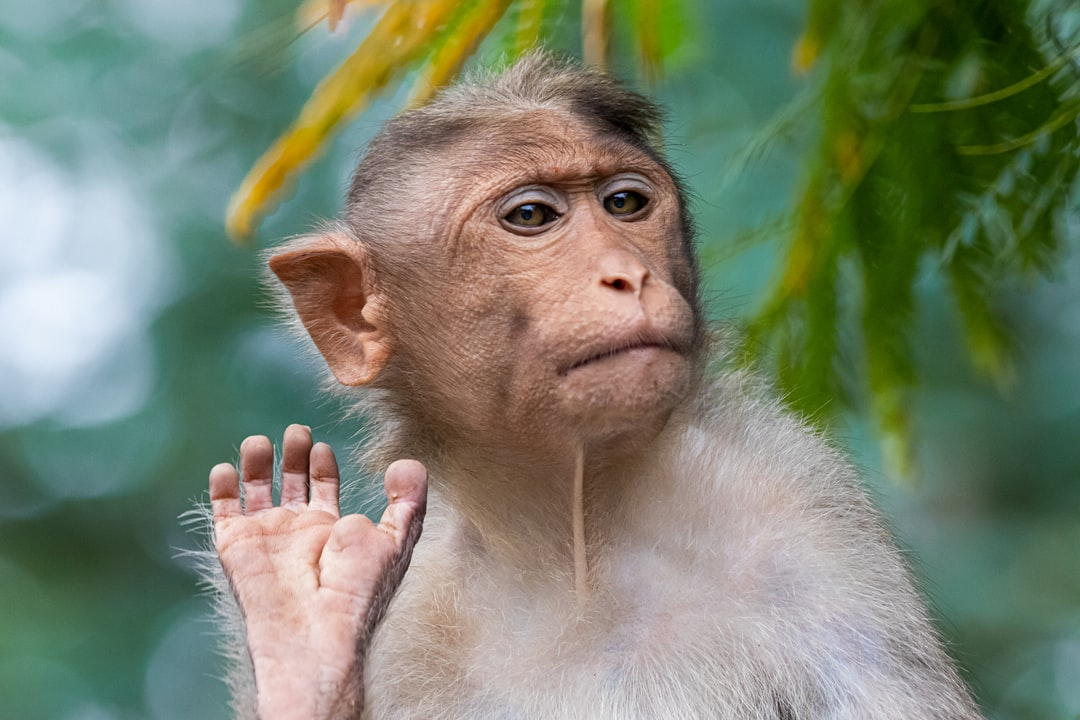
\includegraphics[width=\textwidth]{monkey.jpg}
  \end{minipage}
  \hfill
  \begin{minipage}[b]{0.4\textwidth}
    \caption{This is a sloth}
    \includegraphics[width=\textwidth]{sloth.jpg}
  \end{minipage}
\end{figure}

\begin{figure}[!h]
  \centering
    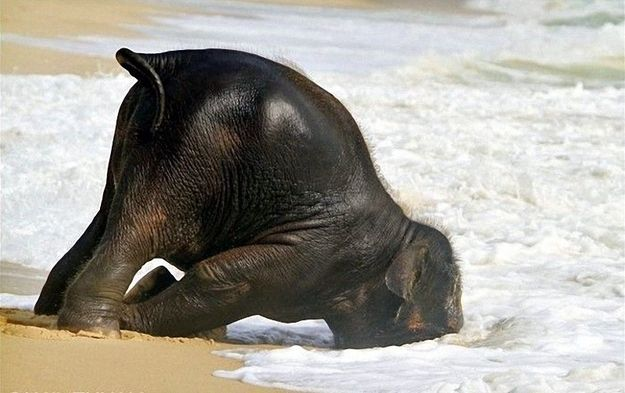
\includegraphics[scale=0.2]{elephant.jpg}
    \caption{This is an elephant}
    \label{fig:elephant}
\end{figure}

This is a label there referes to figure number: \ref{fig:elephant} 

If you want to see the image of figure \ref{fig:elephant} go to page \pageref{fig:elephant} to see it.

\subsubsection{Subsubsection}
This is a subsubsection

\paragraph{This is  paragraph}
Test of paragraph
\subparagraph{This is subparagraph}
Test of subparagraph

\section*{Section without number}

\section{Lists}
\begin{itemize}
  \item Bullet one
  \item Bullet two
\end{itemize}

\begin{itemize}[label={$\ast$}]
  \item Alternative 1
  \item Alternative two
\end{itemize}

\begin{enumerate}
  \item first
  \item second
\end{enumerate}

\renewcommand{\labelenumi}{\Roman{enumi}}
\begin{enumerate}
  \item Roman 1
  \item Roman 2
\end{enumerate}

\section{Table with multiple columns}

This text is a reference to table \ref{table:1} to give an example of how to reference a table
\todo{Make this table better}
\begin{table}[h!]
\begin{center}
  \begin{tabular}{ |l|c|r|c|c|c|c } 
   \hline
   Lefttttttt & Centerrrrrrrr & Rightttttttt &  \multicolumn{2}{c|}{Multi-column} &  \multicolumn{2}{c|}{Multi-Veritcal}  \\  
   \hline
   left2 & cetner1 & right3 & M1 & M2 & \multicolumn{2}{c|}{test}  \\ 
   left3 & center2 & right4 & M3 & M4 & \multicolumn{2}{c|}{test2} \\ 
   \hline
  \end{tabular}
  \caption{This is a table description}
  \label{table:1}
  \end{center}
\end{table}

\section{Code listing}

\UseRawInputEncoding
\begin{lstlisting}[language = Java]
  public static String removeTrailingZeros(double number, boolean isCelcius) {
    String symbol = isCelcius ? "°C" : "°F";
    if (number == (int) number)
        return (int) number + symbol;
    else {
        number = Math.round(number * 100.0) / 100.0;
        return number + symbol;
    }
}
\end{lstlisting}

\section{Math equations}
\todo{Practice some math}
This is an inline math equation: \(x^2 + y^2 = z^2\) \\
Equations on seperate line
\begin{equation}
  2+2=4
\end{equation}
Different math Latex Operations:
\begin{equation}
  \frac{1}{2} \\
\end{equation}
Sum:
\begin{equation}
  \sum_{k=1}3^{-k} = 2 
\end{equation}
Product:
\begin{equation}
  \prod_{k=1}3^{-k} 
\end{equation}
Square root:
\begin{equation}
  \sqrt{25}
\end{equation}
Power:
\begin{equation}
  2^5
\end{equation}
sads
dd
\section{toDo}
\listoftodos

\section{Bibliography}
\nocite{*}
\bibliography{bibloPartTwo.bib}
\bibliographystyle{plain}

\end{document}
